
\subsection{Science Objectives}
\label{sec:science}

\vspace{-0.05in}
 
\subsubsection{The Primordial Universe and Cosmic Inflation}

\vspace{-0.05in}

The observed temperature and E-mode polarization of the \ac{CMB} require primordial inhomogeneities in the gravitational potential, providing a remarkable observational link to the dynamics of the Universe before the hot big bang era. Inflation~\cite{guth81,linde82,albrecht82,sato81,kolb94}, a primordial era of accelerated expansion, provides a compelling 
dynamical origin for the observed statistical homogeneity of the primordial perturbations on even the largest scales. But, Inflation also predicts an as yet unobserved spectrum of primordial gravitational waves sourced directly by 
quantum fluctuations of the tensor component of the metric. 
%The gravitational waves in turn source B-mode polarization in the CMB fluctuations~\cite{kamionkowski97a,zaldarriaga97}. %There are additional degrees of freedom in the primordial metric, the tensor (and vector) modes, that were certainly present in the early universe and whose possible statistics have no known theoretical constraint more restrictive than current observational bounds. 
These gravitational waves make a distinct B-mode imprint on the polarization of the \ac{CMB}. 
Any detection of B-mode polarization, whether generated by the primordial gravitational waves of Inflation ~\cite{kamionkowski97a,zaldarriaga97} or by any other source of early time vector or tensor perturbations, would reveal completely new information about the primordial era. The results would provide significant constraints and consistency checks for current models or could perhaps even overturn them. A detection would have implications far beyond the difficult question of cosmological dynamics by providing evidence for a new scale of particle physics near the GUT scale. In the context of Inflation, the relationship is particularly clear: the potential energy $V$ of the inflaton is related to the tensor-to-scalar ratio $r$ at the peak of the spectrum by $V^{1/4} = 3.7 \times 10^{16} \ r^{1/4}\,\, {\rm GeV}$. 

%In the absence of a detection, a significantly improved upper limit would rule out wide classes of currently consistent models. 
%The observation of a primordial gravitational wave background would generate a revolution in our understanding the origin of our universe and the nature of particle physics, including gravity, at and above the Grand Unification scale of $10^{16}$~GeV.  
%Inflation~\cite{guth81,linde82,albrecht82,sato81,kolb94}, a primordial era of accelerated expansion, provides a compelling 
%dynamical origin for the observed statistical homogeneity of our universe on even the largest scales. 
%Inflation dramatically smoothes away classical inhomogeneities, leaving the inevitable quantum fluctuations 
%of the matter fields and the space-time metric during inflation as the source of structure today.
%%Inflation is consistent with all current astrophysical measurements~\cite{spergel06,Tegmark:2006az,planck2015parameters,planck2015inflation} and is the leading paradigm for the origin of structure in the universe.  
%%The statistics of the primordial curvature fluctuations depend on both the Hubble parameter during inflation and on properties of the matter that sources the fluctuations through the Einstein equation. 
%The predictions of inflation are consistent with an impressive array of observations, including the 
%\ac{CMB} temperature and E-mode polarization and many surveys of the large 
%scale structure of the universe at later times ~\cite{spergel06,Tegmark:2006az,planck2015parameters,planck2015inflation}. 
%But, inflation also predicts an as yet unobserved spectrum of primordial gravitational waves sourced directly by 
%quantum fluctuations of the tensor component of the metric. 
%%The gravitational waves in turn source 
%%B-mode polarization in the CMB fluctuations~\cite{kamionkowski97a,zaldarriaga97}.  

Figure~\ref{fig:clall} shows current data, B-modes from vacuum fluctuations of the metric during an Inflationary 
era for two values of $r$, as well as forecasts for the determination of the \ac{CMB} spectra for EPIC-IM. 
%The large-scale polarization information 
%accessible by a satellite mission is complementary to the smaller scale modes that can be well measured from the ground. 
%The figure also shows the predictions for B-modes from vacuum fluctuations of the metric during an Inflationary era for two values of the tensor-to-scalar ratio $r$. 
For testing inflation, the largest scales $\ell \leq 10$ are particularly important because they reveal 
the presence of B-mode correlations on scales that were super-horizon at the time of recombination~\cite{Lee:2014cya}, 
and because the signal is strongest relative to the B-mode from lensing. A satellite is by far the most suitable 
platform to making the all sky observations necessary to reach the lowest $\ell$'s. 
% In addition, new tests of isotropy on the 
%largest scales can only come from the reionization bump in the E-mode polarization~\cite{}. In its recent report New Worlds New Horizons (NWNH), the decadal survey committee 
%strongly endorsed sub-orbital searches for the B-mode signal from inflation saying that ``The convincing detection of 
%B-mode polarization in the CMB produced in the epoch of reionization would represent a watershed discovery.''~\cite{blandford2010}. 
\begin{figure}[ht!]
%\hspace{-0.2in}
%\parbox{4.in}{\centerline {
%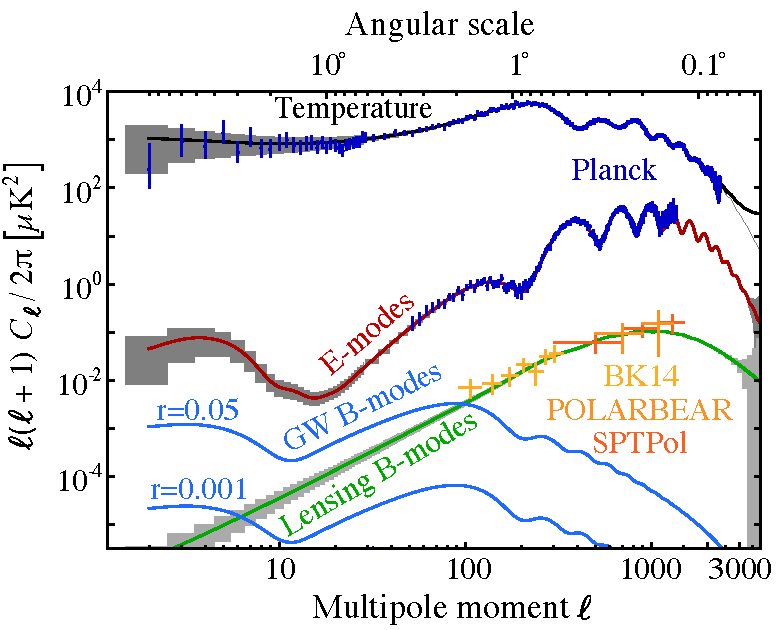
\includegraphics[width=3.5in]{figs/cmb_powspec_v1.pdf}  
%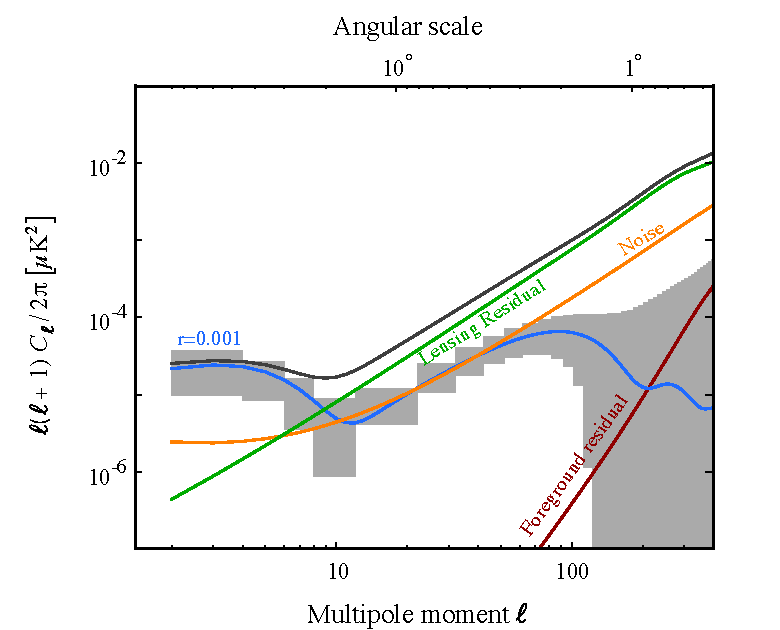
\includegraphics[width=3.5in]{figs/cmbbb_powspec_v1.pdf} } }
%\hspace{0.1in}
%\end{center}
%\parbox{2.5in}{
\begin{center}
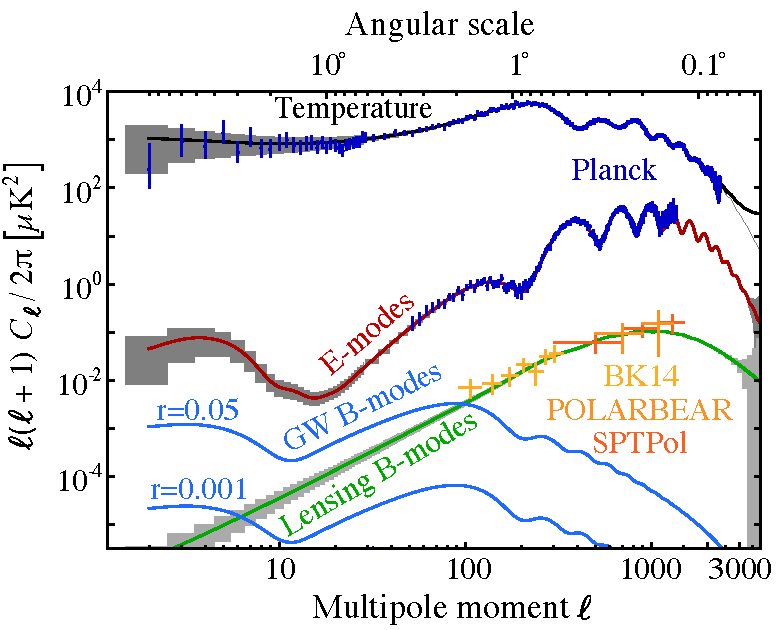
\includegraphics[width=3in]{figs/cmb_powspec_v1.pdf}  
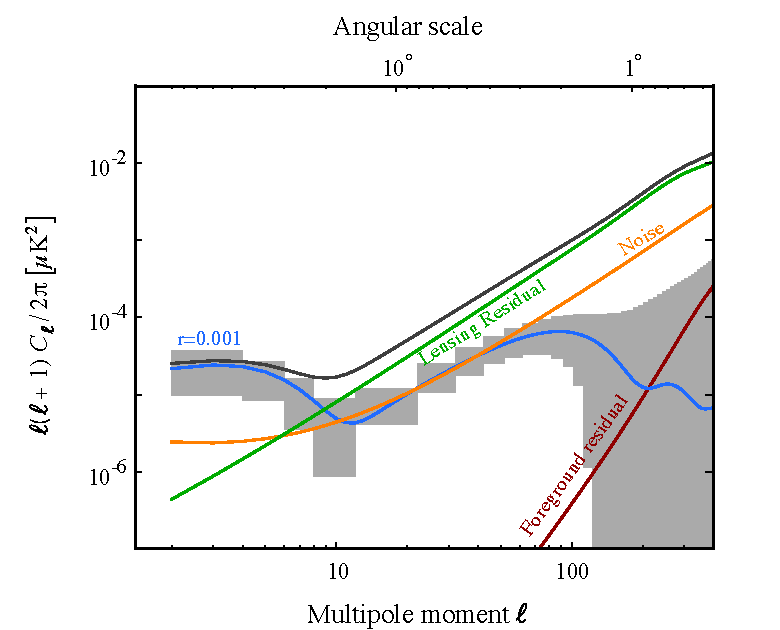
\includegraphics[width=3in]{figs/cmbbb_powspec_v1.pdf}
\end{center}
\vspace{-0.25in}
\caption{ \small \setlength{\baselineskip}{0.95\baselineskip}
Predicted determination of the \ac{CMB} power spectra for EPIC-IM (grey boxes) overlaid
on theoretical predictions (solid lines) and including Planck measurements of the 
temperature and E modes (blue) and of several ground-based measurements 
of the lensing B-modes.  The tensor B-mode predictions (blue) are shown 
for two representative values of the tensor-to-scalar
ratio: $r=0.001$ and $r=0.05.$ 
\label{fig:clall} }
\vspace{-0.05in}
\end{figure}


%In the context of an inflationary primordial universe, a detection of B-modes consistent with the spectrum predicted from vacuum fluctuations would reveal the scale of inflation. The inflationary potential energy $V$ to is related to $r$ at the peak of the spectrum by $V^{1/4} = 3.7 \times 10^{16} \ r^{1/4}\,\, {\rm GeV}$. The observation of a primordial gravitational 
%wave background would generate a revolution in our understanding the origin of our universe and the nature of 
%particle physics, including gravity, at and above the Grand Unification scale of $10^{16}$~GeV.  

In slow roll Inflation 
%Since all inflation models predict primordial B-modes, the space of inflation models can be used to motivate a target sensitivity for future observations. For example, when the slow-roll criteria is met ($\epsilon\equiv-\dot{H}/H^2\ll1$) 
there are just two observationally viable classes of models that naturally explain the measured value of the spectral index $n_s$.
%(by requiring $n_{\rm s}(\mathcal{N})-1\propto-\frac{1}{\mathcal{N}}$, where $\mathcal{N}$ is the number of e-folds between the scale $n_s$ where is observed and end of inflation)~\cite{Mukhanov:2013tua,Roest:2013fha,Creminelli:2014nqa}. 
One is the set of potentials $V(\phi)\propto\phi^p$, which contains many of the canonical inflation models. This 
set is already under significant observational pressure. If the error bars on the spectral index tighten by a factor of about 2, 
and the 95\% C.L. upper limit on $r$ is pushed to even $\sim0.01$, all such models would be ruled out. 
The other class of models includes Starobinsky and Higgs inflation, which both have $r\sim0.003$. A future mission 
capable of reaching $\sigma_r\sim\mathcal{O}(10^{-4})$ would provide significant constraints on nearly every currently favored 
inflation model. The EPIC-IM configuration is forecasted to achieve $\sigma(r)\sim4.8 \times 10^{-4}$ assuming $r=0.01$ 
and no foregrounds. {\bf Check this statement.}
\begin{figure}[ht!]
\hspace{-0.2in}
\parbox{4.in}{\centerline {
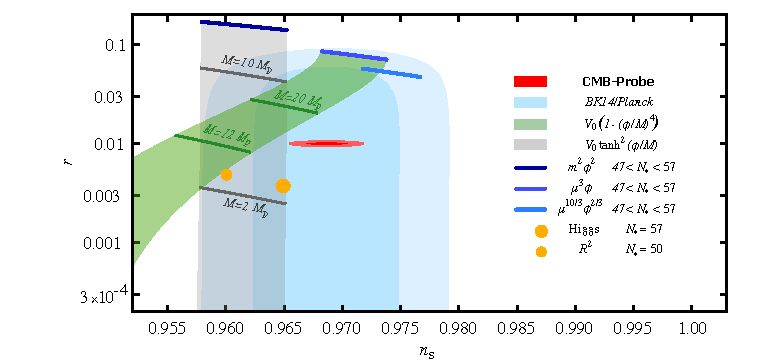
\includegraphics[width=4.5in]{figs/nsrlabeledrp01v1} } }
\hspace{-0.05in}
%\end{center}
\parbox{2.5in}{
\caption{ \small \setlength{\baselineskip}{0.95\baselineskip}
Forecasted constraints in the $n_{\rm s}$--$r$ plane for a fiducial model with $r=0.01$ for EPIC-IM together 
with the current measured 1 and 2$\sigma$ constraints (blue) ~\cite{Array:2015xqh}. Also shown are predictions 
for the models of the inflaton potential discussed in the text: Chaotic inflation for a range of $N_\star$ values (blue lines); 
Higgs and $R^2$ (large and small dots, respectively);  quartic hilltop (green band); and a sub-class of $\alpha$-attractor
models~\cite{Kallosh:2013hoa}
%Constraints on $n_{\rm s}$ are derived from expected CMB-S4 sensitivity to temperature and 
%E-mode power spectra as described in Section~\ref{sec:ttee}. 
%Also shown arecurrent best constraints from a combination of the { BICEP}2/{\em Keck Array} experiments and \planck\ \cite{Array:2015xqh}. 
%Chaotic inflation with $V(\phi)=\mu^{4-p}\phi^p$ for \mbox{$p=2/3,1,2$} are shown as blue lines for $47<N_\star<57$ (with smaller $N_\star$ predicting lower values of $n_{\rm s}$). The Starobinsky model and Higgs inflation are shown as small and large filled orange circles, respectively. The lines show the classes of models discussed in Section~\ref{sec:upperLimits}. The green band shows the predictions for quartic hilltop models, and the gray band shows the prediction of a sub-class of $\alpha$-attractor models~\cite{Kallosh:2013hoa}
\label{fig:nsrp01} } }
\vspace{-0.1in}
\end{figure}

%\begin{figure}[ht]
%\begin{center}
%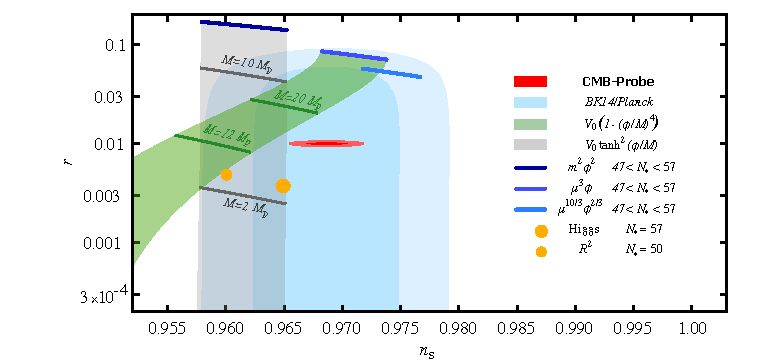
\includegraphics[width=6in]{figs/nsrlabeledrp01v1}
%\end{center}
%\caption{Forecasted constraints in the $n_{\rm s}$--$r$ plane for a fiducial model with $r=0.01$. Constraints 
%on $r$ are derived from {\bf XXX}. Constraints on $n_{\rm s}$ are derived from expected CMB-S4 sensitivity to temperature and 
%E-mode power spectra as described in Section~\ref{sec:ttee}. Also shown are the current best constraints from a combination of the { BICEP}2/{\em Keck Array} experiments and \planck\ \cite{Array:2015xqh}. Chaotic inflation with $V(\phi)=\mu^{4-p}\phi^p$ for \mbox{$p=2/3,1,2$} are shown as blue lines for $47<N_\star<57$ (with smaller $N_\star$ predicting lower values of $n_{\rm s}$). The Starobinsky model and Higgs inflation are shown as small and large filled orange circles, respectively. The lines show the classes of models discussed in Section~\ref{sec:upperLimits}. The green band shows the predictions for quartic hilltop models, and the gray band shows the prediction of a sub-class of $\alpha$-attractor models~\cite{Kallosh:2013hoa}.
%}
%\label{fig:nsrp01}
%\end{figure}

%Forecasts for the capability of a variety of configurations for a future satellite mission (including PIXIE, LiteBird, CORE+, EPIC-2m) are reported to find $\sigma(r)\sim4 \times 10^{-4}$ assuming $r=0.01$, and $\sigma(r)\sim2\times 10^{-4}$ for $r=0$. \
A detection of $B$-modes consistent with a primordial spectrum of vacuum fluctuations would be the first observation of a phenomena directly related to quantum gravity. In addition, any detection with a next generation satellite would be evidence for ``large-field" inflation  \cite{Lyth:1996im}, where a smooth potential that supports inflation extends over a distance in field space $\Delta\phi$ of order $M_p$. 
%It is a generic expectation that quantum gravity requires additional degrees of freedom with masses $M$ near the Planck scale  \cite{}. 
Any inflationary model is necessarily an effective theory valid only below the scale of quantum gravity, but it is a generic expectation that additional heavy degrees (mass $M$) required by quantum gravity \cite{} can easily generate structure in the low-energy potential that limits inflation to $\Delta\phi\lesssim M\sim M_p$. Studies of inflation in string theory have both born out the generic expectation \cite{} and suggested mechanisms to realize large-field inflation \cite{}. A detection of $r$ would therefore provide very strong motivation to better understand how large-field inflation can be naturally incorporated in quantum gravity. 

Inflation generically predicts a B-mode spectrum with the shape shown in Figure \ref{fig:clall}, but inflation need not be correct \cite{} and does not preclude additional sources of $B$-mode polarization either during or after inflation. To be confident of the implications of a detection, the shape and Gaussianity of the B-mode spectrum must be characterized. 
%The standard inflationary prediction is distinguished in these cases by several things: an extremely Gaussian, nearly scale-invariant spectrum with a slight red tilt, the presence of correlations on scales that were not in causal contact at the time of recombination. 
The vast majority of inflation scenarios predict an extremely Gaussian and very nearly scale-invariant, but slightly red, spectrum for gravitational waves. A future satellite mission, combined with Stage 3 ground based observations, could target $\sigma(n_{\rm t})\lesssim1$ at $r=0.01$, for example, to rule out non-vacuum inflationary sources  \cite{Namba:2015gja,Peloso:2016gqs} and physics completely inconsistent with inflation. 
%Post-inflationary phase transitions have been proposed as a non-inflationary source of nearly scale-invariant gravitational waves \cite{Krauss:1991qu,JonesSmith:2007ne,Giblin:2011yh,Figueroa:2012kw,Fenu:2013tea}, but can be distinguished by the absence of super-horizon correlations at the time of recombination. Existing forecasts in the literature \cite{Lee:2014cya} indicate that a ground-based survey alone will not be able to detect super-horizon correlations at high significance if $r$ is much below $0.1$; a satellite will be required.
% A framework to extract specifically this part of the signal was proposed in Ref.~\cite{Baumann:2009mq} and could be applied to robustly extract the component of any signal that must come from physics outside of the hot big bang paradigm. 



%A detection of $B$-modes consistent with a primordial spectrum of vacuum fluctuations would be the first observation of a phenomena directly related to quantum gravity. In addition, evidence for ``large field" inflation would provide strong evidence that the complete theory of quantum gravity must accommodate a Planckian field range for the inflaton. The spectrum of tensor fluctuations depends only on the Hubble parameter $H$ during inflation, while the scalar power depends on both $H$ and the evolution of the homogeneous field sourcing inflation. As a consequence, the tensor-to-scalar ratio $r$ determines the inflaton field range in Planck units (called the ``Lyth bound'' \cite{Lyth:1996im})
%%\begin{equation}
%%\label{eq:Lyth}
%%\frac{\Delta\phi}{M_{\rm P}}=\int_0^{\mathcal{N}_\ast}d\mathcal{N}\,\left(\frac{r}{8}\right)^{1/2}\,,
%%\end{equation}
%%where (applying the general equation to the observationally accessible regime) $\mathcal{N}_\ast$ is the number of e-folds between the end of inflation and the moment when the mode with $k_\ast=0.05\,{\rm Mpc^{-1}}$ (corresponding to the CMB pivot scale) exits the horizon. 
%In many common inflationary models $r$ is a monotonic function of $\mathcal{N}$ so that the tensor-to-scalar ratio at the CMB pivot point $k_*$ is related to the distance the inflaton moves ($\delta\phi$) in Planck units by
%\begin{equation}
%\label{eq:lbound}
%\frac{\Delta\phi}{M_{\rm P}}\gtrsim \left(\frac{r_\ast}{8}\right)^{1/2}\mathcal{N}_\ast\gtrsim \left(\frac{r}{0.01}\right)^{1/2}\,.
%\end{equation}  
%The value of $\mathcal{N}_\ast$ is not well constrained and depends on unknown details of reheating, but $\mathcal{N}_\ast\gtrsim 30$ provides a conservative lower limit, justifying the second inequality in Eq.~(\ref{eq:lbound}). Thus, a tensor-to-scalar ratio $r>10^{-2}$ typically corresponds to a trans-Planckian excursion in field space between the end of inflation and the epoch when the modes we observe in the CMB exit the horizon. The relationship in Eq.~(\ref{eq:lbound}) is significant because it relates the observed amplitude of linearized metric fluctuations to a property of the full quantum field theory for gravity coupled to the inflaton. The action describing inflation, like the action for any other particle physics phenomena, in general will include terms that encode the effects from degrees of freedom that couple to the inflaton, but are too energetic to be probed directly by physics near the inflationary scale. The field range is a measure of the distance in field space over which the corrections from the unknown physics do not significantly affect the low energy dynamics, since otherwise slow-roll inflation would not persist. In theories of quantum gravity we expect degrees of freedom to enter at the Planck scale or below. A field range exceeding the Planck scale would imply that quantum gravity contributions do not have a significant effect over the naively expected scale. A detection of $r$ would therefore provide very strong motivation to better understand how ``large-field inflation" can be naturally incorporated in quantum gravity.

Although the $B$-mode polarization is the richest source of new information, deeper mapping of $E$-mode polarization will also contribute to testing inflationary models. On the largest scales (accessible only from space), $E$-modes will provide new tests of isotropy, while on sufficiently small scales they will allow tighter constraints on the shape of the scalar power spectrum, the amplitude of scalar non-Gaussianities, and isocurvature modes. A satellite mission, combined with next generation ground-based instruments will improve on all measures of the scalar sector by factor of order two.

There is also much to be learned from very small scales. The dissipation of small-scale perturbations through Silk-damping \citep{Sunyaev1970diss, Daly1991, Hu1994, Chluba2012} leads to $\mu$-distortions in the CMB spectrum, which provide a unique means to place stringent constraints on the amplitude of the small-scale curvature power spectrum. This information is on small scales (wavelength $0.1 \,{\rm kpc} \lesssim \lambda \lesssim 1\, {\rm Mpc}$) and from early times ($10^4 \lesssim z\lesssim 10^6$), inaccessible through any other observation. In $\Lambda$CDM \citep{Chluba2016LCDM}, distortions are predicted at a level of $\mu=(2.0\pm0.14)\times 10^{-8}$. A detection would deliver a complementary test for the inflation paradigm~\citep{Chluba2012inflaton, Dent2012, Chluba2013PCA, Clesse2014, Cabass2016}, and new probes of the particle spectrum of inflation through new tests of non-Gaussianity ~\citep{Pajer2012, Ganc2012, Biagetti2013, Razi2015}. Precise measurements of signals at this level will be extremely challenging and requires unprecedented control of systematics and modeling of foregrounds. It would also bring us to the sensitivity level required to detect the cosmological recombination radiation \citep{Sunyaev2009, Chluba2016} imprinted by the recombination of hydrogen and helium at redshift $z\simeq 10^3-10^4$, which can be used to probe the physics of recombination. Optimizing next-generation CMB spectrometers for these purposes requires extensive studies.
%In summary, a detection of primordial gravitational waves consistent with the standard inflationary prediction would reveal the presence of a new fundamental energy scale for particle physics and would have far reaching implications for quantum gravity. Detecting correlations on the largest scales would confirm a primordial origin. Any departure from a nearly scale-invariant, nearly Gaussian spectrum would reveal new physics beyond the simplest inflationary model. In the absence of a detection, an improvement by about two orders of magnitude on the current upper limit would qualitatively change how we think about the inflationary paradigm.

%\comred{{[\sc distortion part does not link to what is written before yet. The text before has to be worked over significantly to make that match.]}} Another clear target is predicted by the dissipation of small-scale perturbation through Silk-damping \citep{Sunyaev1970diss, Daly1991, Hu1994, Chluba2012}. This process allows us to place stringent constraints on the amplitude of the small-scale curvature power spectrum, present at scales (wavelength $0.1 \,{\rm kpc} \lesssim \lambda \lesssim 1\, {\rm Mpc}$) and epochs ($10^4 \lesssim z\lesssim 10^6$) inaccessible through any other observation. It delivers a complementary test for the inflation paradigm~\citep{Chluba2012inflaton, Dent2012, Chluba2013PCA, Clesse2014, Cabass2016}, with $\mu=(2.0\pm0.14)\times 10^{-8}$ expected in $\Lambda$CDM \citep{Chluba2016LCDM}. Precise measurements of signals at this level will be extremely challenging and requires unprecedented control of systematics and modeling of foregrounds. It would also bring us to the sensitivity level required to detect the cosmological recombination radiation \citep{Sunyaev2009, Chluba2016} imprinted by the recombination of hydrogen and helium at redshift $z\simeq 10^3-10^4$, which can be used to probe the physics of recombination. Anisotropy in the $\mu$-distortion can furthermore be created through `ultra-squeezed limit' non-Gaussianity~\citep{Pajer2012, Ganc2012} and can be used to probe scale-dependent non-Gaussianity~\citep{Biagetti2013, Razi2015}. Optimizing next-generation CMB spectrometers for these purposes requires extensive studies.
%
\vspace{-0.15in}

\subsubsection{Light Relics and Dark Matter}

\vspace{-0.05in}

After inflation, the universe was reheated to temperatures of at least 10 MeV and perhaps as high as $10^{10}$ GeV.  
At these high temperatures, even very weakly interacting or very massive particles, such as those arising 
in extensions of the Standard model of particle physics, can be produced in large abundances.  As the universe expands and cools, 
the particles fall out of equilibrium and leave observable signatures in the \ac{CMB} power spectra. 
%primary CMB or through gravitational lensing.  
Through these effects the CMB is a sensitive probe of neutrino properties and of other 
candidate light particles.  

Much of the information about our thermal history and the particle content of the universe is encoded in the $T$ and $E$ power spectra.  
A high-precision measurement of these spectra over the full sky is expected to significantly improve our understanding of the post-inflationary 
universe.  This is particularly true in $E$-mode polarization where, to date, far fewer modes have be measured at the level of cosmic variance than in temperature.

%The spectra at high-$\ell$ contain important information about the components of the thermal plasma and their interactions around the time of recombination.  
One particular compelling target is the effective number of neutrino species $\Neff$, which parameterizes the total amount of energy density in radiation 
at the time of recombination. Despite its common name, $\Neff$ encodes the total number of light relic particles.  The canonical value with three species of 
neutrinos is $\Neff = 3.046$. 
%It is defined such that in the Standard model of particle physics with normal thermal evolution, $\Neff = 3.046$ due to the energy density 
%in the three species of neutrinos.  
%$\Neff$ is also sensitive to any additional light relic particles as their gravitational influence is identical to the neutrinos.  
%In fact, if there was an 
Additional light particles 
%in thermal equilibrium with the Standard model particles at any point in our history, it will 
contribute a change to $\Neff$ of at least $\Delta \Neff \geq g \, 0.027$ where $g \geq 1$ is the number of degrees of freedom of the new particle~\cite{Brust:2013xpv,Baumann:2016wac}.  
This defines a compelling target of $\sigma(\Neff) < 0.027$ for future CMB observations.  New light particles are a common feature of many 
approaches to physics
beyond the Standard model and are directly tied to some of the most significant problems in the Standard model.  
Either a limit or detection of $\Delta \Neff$ at this level would provide a powerful insight into the fundamental laws of nature. 

The presence of free-streaming radiation changes the detailed features of the $TT$, $TE$ and $EE$ spectra at all $\ell$.  
In particular, it changes the locations of the acoustic peaks and alters the damping tail at high-$\ell$~\cite{Bashinsky:2003tk,Hou:2011ec,Follin:2015hya,Baumann:2015rya}.  Similar changes to the spectra 
arise from many other compelling targets including the helium fraction $Y_p$ and more general dark sector physics.  For this reason, 
constraints on $\Neff$ a useful proxy for the information available in the high-$\ell$ power spectra.  

Forecasts for $\Neff$ are shown in the right hand panel of Figure~\ref{fig:Neff_future}.  The two most important quantities for improving 
constraints on $\Neff$ and other high-$\ell$ targets are the fraction of sky observed $f_{\rm sky}$ and the noise temperature. Both are 
specific strengths of a space mission. The EPIC-IM mission reaching 
an effective noise temperature noise of 0.9 $\mu$K-arcmin over the full sky gives competitive constraining power when compared other proposals.  
The full-sky nature of the proposed mission would allow for cosmic variance limited $E$-modes over most of the sky and a large range of $\ell$.

The main downside of a space-based mission is that we cannot reach the resolutions available from the ground.  However, 
we see that at 5' resolution and 1 $\mu$K-arcminute noise the forecasts are less sensitive to the resolution then one might naively 
expected.  In particular we can reach $\sigma(\Neff) < 0.035$ for temperature noise from 1-2 $\mu$K-arcmin and $f_{\rm sky} =0.6-0.8$.  
These forecasts are competitive with CMB Stage IV.  Specifically, the larger sky fraction and sensitivity available from space appears 
to compensate for the reduced resolution.  In fact, the full sky measurement would provide complimentary information that could be 
combined with ground based surveys to further improve over the limits available from either experiment.  This is particularly important for 
$\Neff$ which is tantalizingly close to the target of $\sigma(\Neff) =0.027$ and therefore even an apparently modest improvement 
could have a major scientific impact.  

%Neutrino properties measurements in accelerator give a minimum value of $\sum m_\nu =58$.  
%that is accessible from Cosmology.  
%The most distinctive feature of $\sum m_\nu$ is that it suppresses the growth of structure on small scales.  This suppression
%can be measure in the CMB through amplitude of the lensing power spectra compared to the primary CMB.  In principle, 
%this relative difference can yield a measurement  of the minimum value of $\sum m_\nu =58$ meV at 4-5 $\sigma$ for a 
%number of future cosmological surveys.  However, sensitivity to $\sum m_\nu$ is ultimately limited by our knowledge of 
%the primordial amplitude of fluctuations $A_s$ which is strongly degenerate with the optical depth $\tau$. 

%The current limit on $\tau$ from the Planck satellite of $\tau = 0.055 \pm 0.009$ ultimately limits 
%$\sigma(\sum m_\nu) \gtrsim 25$ meV, as shown in the panel of Figure~\ref{fig:Neff_future}.  While the figure 
%shows the sensitivity of a space-based CMB mission to $\sum m_\nu$, this lower limit is common to any 
%measurement that depends on the relative suppression.  Therefore, a cosmological detection of 
%$\sum m_\nu = 58$~meV at 3-5 $\sigma$ depends crucially on an improvement measurement of $\tau$.  
%To date, the only proven method for such a measurement is from a space-based CMB observations.  The best 
%constraints on $\tau$ come from $E$-modes with $\ell < 20$ which requires control over the largest angular scales.  


\begin{figure}[t!]
\begin{center}
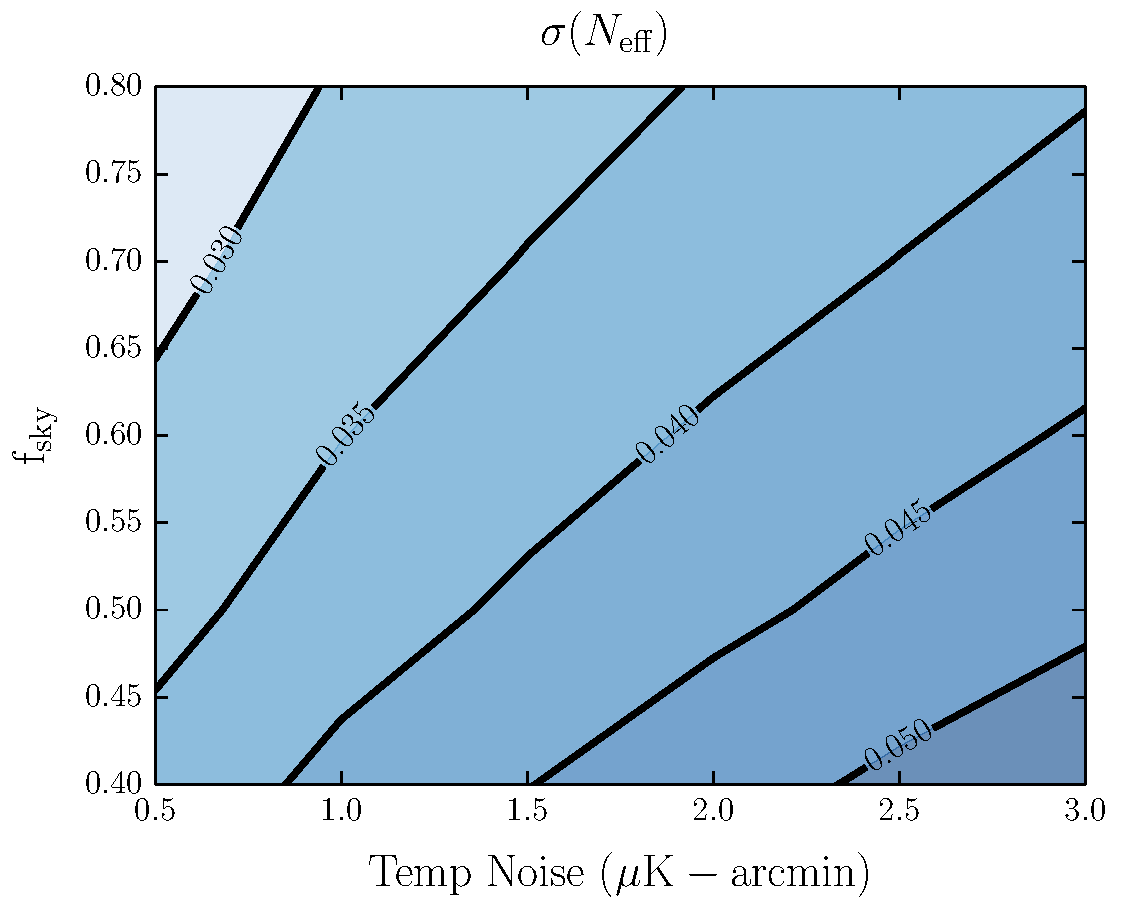
\includegraphics[width=0.45\textwidth]{figs/Neff.pdf}
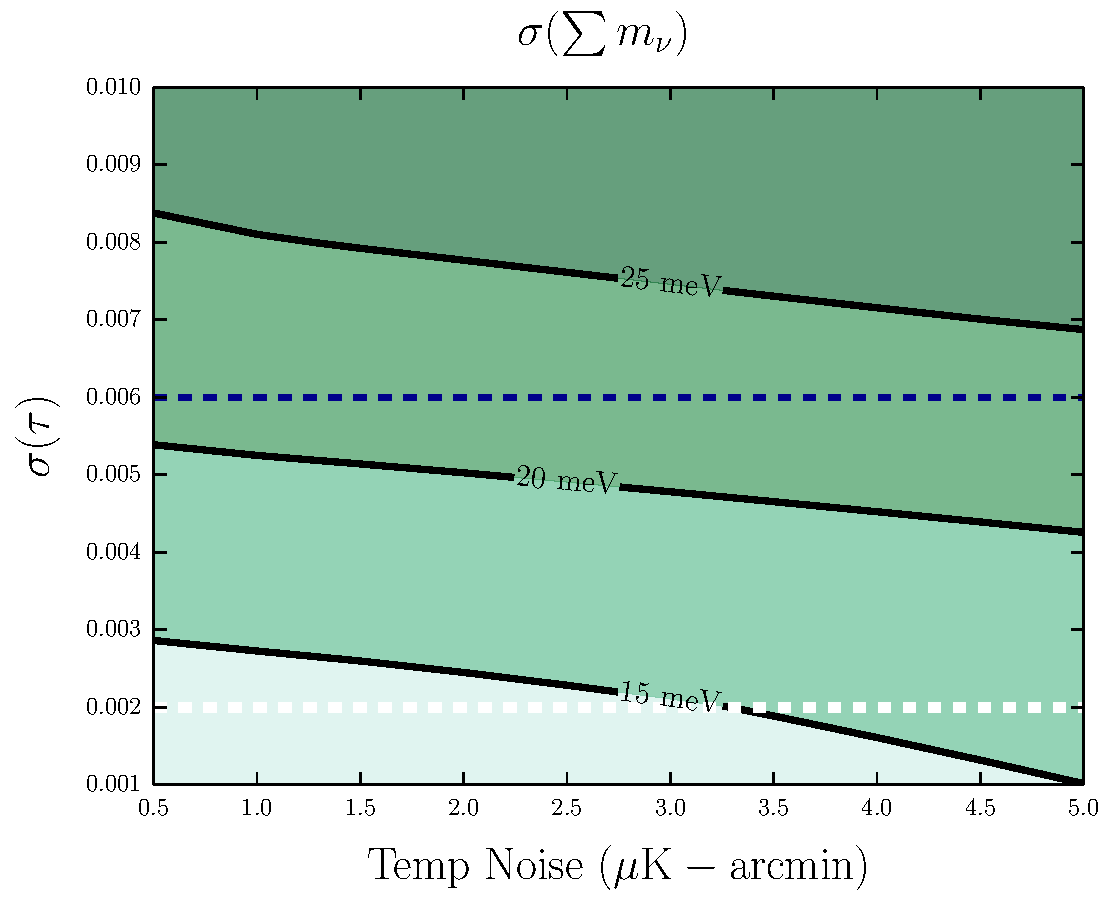
\includegraphics[width=0.45\textwidth]{figs/Mnu_tauprior.pdf}
\caption{ \small \setlength{\baselineskip}{0.95\baselineskip}
$\Neff$ as a function of noise and sky fraction assuming 5' resolution (left) and
Neutrino mass constraints as a function of uncertainties in measurement of $\tau$ and noise for a 5' beam and 
sky fraction of $f_{\rm sky} = 0.7$. 
Vertical lines denote the expected performance of EPIC-IM. 
The blue dashed line is the current \planck limit; the grey dashed line is the limit from cosmic variance 
measurement of $\tau$. All forecasts assume internal delensing of the $T$ and $E$-maps~\cite{Green:2016cjr}, including residual non-Gaussian covariances.
\label{fig:Neff_future} }
\end{center}
\vspace{-0.15in}
\end{figure}

Measurements of the primary CMB and CMB lensing are very sensitive to particles with long-lifetimes that service 
until the era of recombination.  Furthermore, the primary CMB is indirectly sensitive to BBN through the helium fraction, $Y_p$, 
that can be detect energy injections at those times.  However, many relics of the early universe are not cosmologically stable but 
can survive beyond the time of BBN.  Energy injection between the two eras is not directly captured by the CMB anisotropies 
but can be tested by BBN consistency of $Y_p$ with the measured value of $\Neff$~\cite{Fischler:2010xz,Baumann:2015rya}.  

Additional, far more sensitive measurements of this intermediate era are possible through the {\it distortions} of the 
CMB black-body spectrum. This will allow us to place stringent bounds on the presence of long-lived decaying 
particles \citep{Hu1993b, Chluba2013fore, Chluba2013PCA, Dimastrogiovanni2015} and other non-standard 
physics, such as axions, primordial magnetic fields and superconducting 
strings \citep[e.g.,][]{Jedamzik2000, Tashiro2012, Dolgov2013, Tashiro2013, Caldwell2013}.


Through cosmological measurements, we have already confirmed the existence of one relic that lies beyond the Standard Model: dark matter.  Characterizing the nature of dark matter is one of the most basic problems in cosmology and astro-particle physics.  For a conventional WIMP candidate, the CMB places very stringent constraints on dark matter through possible energy injection at the time of recombination.  A thermal relic will necessarily annihilate into Standard model particles which distorts the Thomson visibility function and ultimately the shape of the primary $T$ and $E$ spectra \citep{Peebles2000, Chen2004, Padmanabhan2005}.  A dark matter candidate can also have a slow decay to Standard models particles which is similarly constrained by the CMB~\cite{Slatyer:2016qyl}.

A somewhat more model-independent approach is to constraint dark matter interactions that would effect the evolution of the effective dark matter fluid and its interactions with baryons or photons.  The simplest example is to constraint the baryon-dark matter cross section through its effective coupling of the two fluids~\cite{Dvorkin:2013cea}.  These couplings effect the evolution of fluctuations and ultimately the $T$ and $E$ spectra.  More exotic dark sectors can produce a rich phenomenology in the CMB and in the large-scale structure without necessarily producing an associated signature in direct detection experiments or indirect searches (e.g.~\cite{Cyr-Racine:2013fsa,Buen-Abad:2015ova,Lesgourgues:2015wza}). 

Interactions of DM with standard model particles can also be constrained through CMB spectral distortions \citep{Yacine2015DM}. As the Universe expands, the matter cools. Compton interactions with electrons keep the normal matter at the CMB temperature until well after recombination. This leads to a small distortion of the CMB with a negative chemical potential \citep{Chluba2011therm}. In a similar manner, interactions of DM with electron, protons or directly with CMB photons can lead to a distortion. These constraints could be strongly improved with future CMB spectroscopy \citep{Yacine2015DM}.

\vspace{-0.15in}

\subsubsection{Neutrino Mass}

\vspace{-0.05in}

One of the last unknowns of the Standard model of particle physics is the absolute mass scale of the neutrinos.  While measurements of neutrino oscillations demonstrate the neutrinos have mass, directly measuring the scale of the masses is challenging experimentally.  Current measurement of $\Neff$ confirm the existence of a cosmological abundance of neutrinos whose gravitational influence is detectable in the CMB and in large scale structure.  Cosmology presents a unique opportunity to measure the the sum of neutrino masses $\sum m_\nu$ through the suppression of the growth of structures in the Universe on small scales.  In fact, the CMB allows for an internal measurement $\sum m_\nu$ by comparing the amplitude of the lensing power spectrum to that of the other CMB spectra~\cite{Kaplinghat:2003bh}.

%Larger $\sum m_\nu$ gives a larger suppression and the $\sum m_\nu$ can be measured by 

The \ac{CMB} Probe would be a valuable tool in the quest for a cosmological detection of $\sum m_\nu$.   The sensitivity to $\sum m_\nu$ from suppression of power alone is limited by our knowledge of 
the primordial amplitude of fluctuations $A_s$ which is strongly degenerate with the optical depth $\tau$.  The current limit on $\tau$ from \planck\ of 
$\tau = 0.055 \pm 0.009$~\cite{} limits 
$\sigma(\sum m_\nu) \gtrsim 25$ meV; see Figure~\ref{fig:Neff_future}.  
%This lower limit is common to any measurement that depends on the relative suppression.  
Therefore, a detection of the minimum value expected from particle physics  
$\sum m_\nu = 58$~meV at 3-5 $\sigma$ depends crucially on an improvement measurement of $\tau$.  

To date, the only proven method for such a measurement is from a space-based CMB observations.  The best constraints on $\tau$ come from $E$-modes with $\ell < 20$ which requires control over the largest angular scales.  The \ac{CMB} Probe could, in principle, reach the cosmic variance limit of $\tau \sim 0.002$ and could reach $\sigma(\sum m_\nu) < 15$ meV when combined with DESI BAO.  A detection of $\sum m_\nu$ at this level is not possible with any existing survey without an improvement to the measurement of $\tau$.


\vspace{-0.15in}

\subsubsection{Cosmological structure formation}

\vspace{-0.05in}

Understanding the evolution of cosmological structures from the formation of the
first stars to the present time is a key goal of cosmology \citep{dunlop2011}.


In particular understanding cosmological reionization, the transformation of neutral
hydrogen into an ionized state, and establishing a connection between reionization and early galaxies, will 
reveal valuable information about the star formation history and the physical processes that formed the galaxies of various luminosities and masses we see today. 
 Though a number of diverse observational probes have rendered a preliminary picture of the reionization epoch, details of the transition from the neutral to ionized 
 Universe are still the subject of intense activity. 
In the current picture, early galaxies reionize hydrogen progressively throughout the entire Universe between $z = 12$ and $z  = 6$,
while quasars take over to reionize helium from $z \simeq 6$ to $z \simeq 2$. However many questions remain. When did the epoch of reionization
(EoR) start, and how long did it last? Are early galaxies enough to reionize the entire Universe or is another source required?
To answer these questions one can resort to using the traces left by the EoR in the cosmic microwave background (CMB) anisotropies.
More specifically, the integrated Thomson scattering optical depth, $\tau$, due to the scattering of CMB photons off free electrons after reionization, 
as inferred from the polarised CMB photons. 
The optical depth to reionization, $\tau$, places an important integral constraint on the extended reionization history.
The {\it Planck} Collaboration~\cite{planck2015-XLVI,planck2015-XXXI} reported recently a value of $\tau=0.055 \pm 0.009$ significantly lower than previous estimates. 
This suggests that an early onset of reionization is strongly disfavoured by the {\it Planck} data. 
The {\it Planck} Collaboration~\cite{planck2015-XXXI} showed that this result reduces the tension between CMB-based analyses and constraints from 
other astrophysical sources. 
A cosmic variance limited measurement of E-mode polarization on large scales, possible with a probe mission, will render the most accurate 
determination of $\tau$ (Figure~\ref{fig:Neff_future}
shows a cosmic variance limit measurement of $\tau$ along with the current {\it Planck} limit, break the degeneracy with the neutrino mass, 
set stringent constraints on models of the reionization epoch, and, finally, help understanding the formation of the cosmological structures we see today.


The anisotropies in the Cosmic Infrared Background (CIB), produced by
dusty star-forming galaxies (DSFGs) in a wide redshift range, are
an excellent probe of both the history of star formation and the link between
galaxies and dark matter across cosmic time. The {\it Planck} Collaboration \citep{planck2014-XXX,planckXVIII},
derived values of the star formation rate density that,
at redshifts z$\mathrm{\sim3}$, are about three times higher
than constraints from number counts measurements (\cite{madau2014}).
The new mission probe, by measuring CIB anisotropies with 100 times more
sensitivity than {\it Planck}, will be able to shed light on this intriguing
discrepancy. In particular, it will be possible to constrain the global star formation rate (SFR)
with one tenth of {\it Planck}'s uncertainty
at z$\mathrm{=3}$. Moreover, it will be possible to identify and constrain a
characteristic halo mass $M_{\mathrm{eff}}$,
which determines the most efficient gas accretion and SFR, and
therefore sets the evolution of the galaxies residing within
a dark matter halo. Current models and measurements
constrain this characteristic halo mass at
$M_{\mathrm{eff}}\sim 10^{12}$ solar masses with about $\mathrm{10\%}$
uncertainty, while the new mission probe will
constrain this parameter at the percent level.\\
Moreover, because DSFGs trace the underlying dark matter
field in a broad redshift range, the CIB will
correlate with multiple dark matter
tracers such as catalogs of galaxies and quasars
\citep{serra2014,wang2015},
and diffuse maps of the $\gamma$-ray and
the X-ray background \citep{cooray2016}.
These cross-correlations will provide an additional probe of the
global star formation history, and they
will shed light on the interaction between light and matter
in a broad wavelength range.

Large-scale structure can also be probed using CMB spectral distortions measurements. In fact, the largest guaranteed distortion is caused by the associated late-time energy release of forming structures and from reionization \citep{Sunyaev1972b, Hu1994pert, Oh2003, Cen1999, Refregier2000}, imprinting a $y$-type distortion 
with $y \simeq 2\times 10^{-6}$ \citep[e.g.,][]{Refregier2000, Hill2015}. This distortion is only one order of magnitude below the current limit from COBE/FIRAS and, even with most pessimistic assumptions about foregrounds, should be clearly detected with the next-generation spectrometers we propose to study. A detection will give information about the total energy output of first stars, AGN and galaxy clusters. In particular, group-size clusters that have masses $M\simeq 10^{13}\,M_{\odot}$ contribute significantly to the signal. With temperature $k T_{\rm e}\simeq 1\,{\rm keV}$ these are still sufficiently hot to create a detectable relativistic temperature correction to the large $y$-distortion, 
which can be used to constrain the currently uncertain feedback mechanisms used in hydrodynamical simulations
of cosmic structure formation~\citep{Hill2015}. These two inevitable signals probe the low-redshift 
Universe and provide clear targets for future spectral distortions measurements and their requirements in the presence of foregrounds.

The CMB spectrum varies spatially across the sky. One source of such anisotropic distortion is related to clusters of galaxies and has already been measured by Planck~\citep{Planck2013SZ}. A combination of precise CMB imaging and spectroscopic measurements will allow observing the relativistic temperature correction of individual SZ clusters~\citep{Sazonov1998, Itoh98, Challinor98}, which will calibrate cluster scaling relations and inform our knowledge of the dynamical state of the cluster atmosphere. Finally, resonant scattering signals in the recombination \citep{Jose2005, Carlos2007Pol, Lewis2013} and post-recombination eras \citep{Kaustuv2004, Schleicher2008} can lead to spectral-spatial CMB signals that can be used to constrain the presence of metals in the dark ages and the physics of recombination. For all these applications, instrumental synergies between CMB imaging and spectroscopy need to be studied in detail. 



These studies will be key to address three of the seven key questions identified in the Astro2010 report ``New Worlds, New Horizons in Astronomy and Astrophysics'' (NAS Decadal Survey, p. 47): {\it What is the fossil record of galaxy assembly                                                                               
from the first stars to present? What are the connections between dark and luminous matter? How do cosmic structures form and evolve?}



%\begin{figure}[htbp!]
%\hspace{0.in}
%\parbox{4.2in}{ \centerline {
%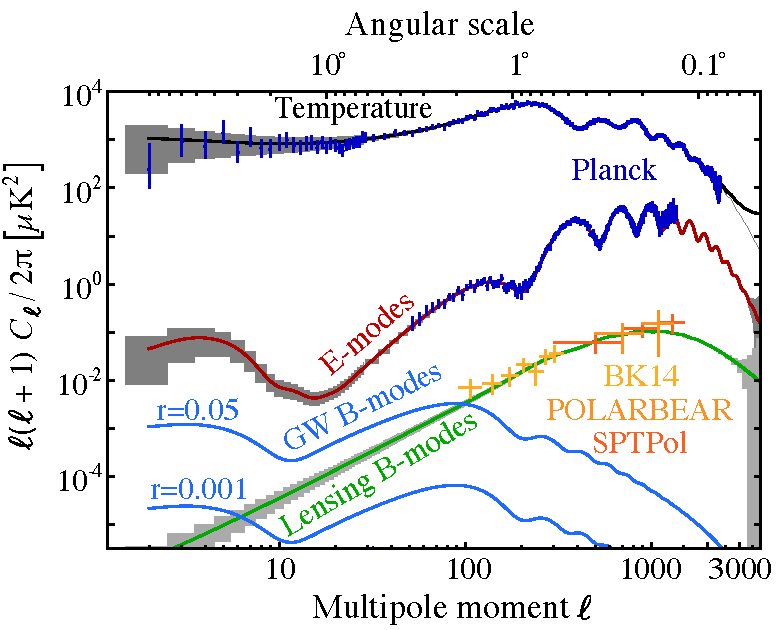
\includegraphics[width=2.0in] {figs/cmb_powspec_v1.pdf}  
%\hspace{0.1in}
%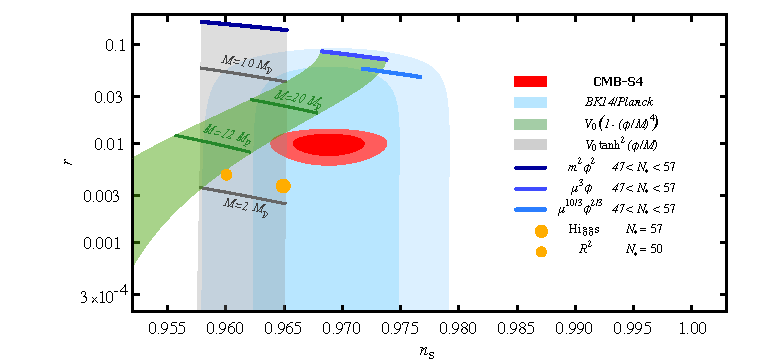
\includegraphics[width=2.0in] {Figures/nsrlabeledrp01v10s}  }  }
%\hspace{0.1in}
%\parbox{2.in}{
%\caption{ \small \setlength{\baselineskip}{0.90\baselineskip}
%    Theory and observations for the spectrum; Space of predictions from important classes of inflation models.
%\label{fig:inflation} } }   
%\vspace{-0.05in}
%\end{figure}


%A significant contamination of CMB anisotropy maps is due to
%the foreground emission from infrared (IR)
%galaxies, responsible for the cosmic infrared background (CIB).
%The CIB is the second largest
%extragalactic background after the CMB, with an approximate
%brightness of 24 nW m$\mathrm{^{-2} sr^{-1}}$ \citep{dole2006}.

%Dust enshrouded star-forming galaxies at redshift $\mathrm{z\sim 1-3}$ is heated by starlight at ultraviolet (UV) and optical wavelengths,
%and re-radiates at mid-IR to sub-millimetre wavelengths. This emission, from galaxies actively
%producing stars at their peak of star formation, reaches us in the far-infrared (FIR) regime as the cosmic infrared
%background (CIB). The CIB carries a wealth of information about the history of star formation and dark matter 
%in the Universe, and will be used to constrain foreground levels and to remove the effects of lensing 
%from the CMB polarization signals. 

%With a brightness of 24 nW m$\mathrm{^{-2} sr^{-1}}$ \citep{dole2006}, it is 
%the second most intense extragalactic background after the CMB. 
%While the CIB is not our only handle on the evolution of the
%cosmic star formation rate (SFR), it is particularly important
%because FIR/sub-millimetre surveys are not subjected to some
%uncertain steps in the conversion from galaxy counts and luminosities to SFRs,
%affecting, e.g., optical surveys.

%The drawback of working with a
%high density of faint, distant sources in the FIR regime is that
%individual objects are blended. While both the {\it Herschel} and {\it Planck} satellites
%recently performed ground-breaking measurements of the CIB
%\citep{amblard2011,viero2013a,planck2014-XXX,mak2016}, only a
%negligible fraction of {\it Planck} sources have been individually
%identified, due to its poor angular resolution, while for
%{\it Herschel} maps, only 10$\%$ of the objects
%has been resolved into individual galaxies at 857 GHz \cite{bethermin2010}.
%However, the anisotropies detected in the
%unresolved background can be analyzed through statistical tools
%such as the angular power spectrum \citep{knox2001} and, since they trace the
%underlying dark matter field, they can be interpreted with
%phenomenological models linking dark matter halos to IR galaxies,
%such as the Halo Model \cite{cooray2002,shang2012}.

%{\bf Star Formation History:}
%The Planck Collaboration, analyzing CIB anisotropy and its correlation with CMB lensing \citep{planck2014-XXX,planckXVIII},
%derived limits on the star formation rate that
%at redshift $\mathrm{z>2}$ are higher than with other datasets (see for example \cite{madau2014}) 
%\comred{by how much higher?}. With \comred{100?} times  the Planck sensitivity at \comred{??} GHz, 
%\comred{the constraints on the star formation rate will improve by ??}
% Clearly, more accurate measurements of the CIB clustering at the
% angular scales probed by {\it Planck} will be extremely useful to
%gain more insight on the evolution of the star formation rate at
% high redshift. 
%The new mission probe will measure CIB anisotropies
%with only one tenth of {\it Planck}'s instrumental noise at the critical
%scales where the clustering of galaxies in the same dark matter
%halo (the 1-halo term) has the same amplitude as the
%clustering due to galaxies in separated halos
%(the 2-halo term). Assuming a precise knowledge of the Poisson level of CIB
%galaxies, we will be able to firmly constrain our models of CIB clustering,
%and thus address three of the seven key questions
%identified in the Astro2010 report ``New Worlds, New Horizons in Astronomy and Astrophysics''
%(NAS Decadal Survey, p. 47): {\it What is the fossil record of galaxy assembly                                                   
%from the first stars to present? What are the connections                                           
%between dark and luminous matter? How do cosmic structures form and evolve?}
%\comred{deliverables from previous paragraph not clear} 

%{\bf Dark Matter:}
%The CIB, being a tracer of the dark matter field over a broad redshift range,
%can be cross-correlatated with many other datasets to explore
%the interplay between CIB galaxies and dark matter. examples include the cross-correlations
%with catalogs of quasars \citep{wang2015} and
%galaxies \citep{serra2014} to constrain the interplay between
%SFR and halo mass, and the cross-correlation with the Cosmic
%$\mathrm{\gamma}$-ray background from {\it Fermi}-LAT
%\citep{fermi2016} to constrain the dark matter annihilation
%cross-section \citep{cooray2016}.
%\comred{what are the quantitative outcomes of these cross-correlations}
%Beyond the
%cross-correlation with the lensing of the CMB
%\citep{planckXVIII,holder2013}, some other 

%{\bf CMB Delensing:} Since they are both tracers of the underlying mass distribution over
%a broad range of redshifts, the CIB and CMB lensing are highly correlated
%\citep{planckXVIII}. In particular, the CIB can be used as
%an ideal proxy for the CMB lensing field in delensing studies, aiming at
%reducing the confusion due to B-modes from lensing in the search of the
%signal from primordial gravitational waves.
%Recently \cite{sherwin2015,larsen2016} showed that co-adding {\it Planck} CIB maps
%greatly improves the delensing performance. Upcoming CMB surveys
%will heavily rely on delensing methods for constraining the
%inflationary B-mode polarization signal, and CIB delensing of temperature and E-mode
%polarization might also help improving constraints on other parameters such as the effective
%number of neutrino species $\mathrm{N_{eff}}$ \citep{larsen2016}.
%\comred{can we be quantitative}

%{\bf CMB Foregrounds:} The Planck collaboration found that the CIB is 
%a significant contributor to foregrounds in the 143x217 and 217x217 GHz 
%band correlations~\citep{planck2016like}. Both the clustering and Poisson components of the 
%CIB were found to be important. The cross-correlation between IR galaxies and the thermal
%Sunyaev-Zeldovich (tSZ) effect provides an additional contamination. 
%Thus, an accurate determination of both CIB and CIB-tSZ power
%spectra will be extremely useful when accounting for these foregrounds
%in the CMB parameter estimation.
%\comred{make quantitative?} 

%However, constraining the history of star formation is not the only reason for measuring CIB anisotropies with increased sensitivity from very large to very small scales. Below, we briefly discuss some others. 
%\begin{itemize}
%\item The CIB is an important foreground for CMB studies. As shown in \cite{planck2016like}, a significant contribution to the astrophysical foreground in the 143x217 and 217x217 GHz channels is due to both the clustering and Poisson components of the CIB. The cross-correlation between IR galaxies and the thermal Sunyaev-Zeldovich (tSZ) effect provides an additional contamination. Thus, an accurate determination of both CIB and CIB-tSZ power spectra will be extremely useful when accounting for these foregrounds in the CMB parameter estimation.
%\item The CIB, being a tracer of the dark matter field over a broad redshift range, can be cross-correlatated with many other datasets to explore the interplay between CIB galaxies and dark matter. Beyond the cross-correlation with the lensing of the CMB \citep{planckXVIII,holder2013}, some other examples include the cross-correlations with catalogs of quasars \citep{wang2015} and galaxies \citep{serra2014} to constrain the interplay between SFR and halo mass, and the cross-correlation with the Cosmic $\mathrm{\gamma}$-ray background from {\it Fermi}-LAT \citep{fermi2016} to constrain the dark matter annihilation cross-section \citep{cooray2016}.
%\item Since they are both tracers of the underlying mass distribution over
%a broad range of redshifts, the CIB and CMB lensing are highly correlated
%\citep{planckXVIII}. In particular, the CIB can be used as
%an ideal proxy for the CMB lensing field in delensing studies, aiming at
%reducing the confusion due to B-modes from lensing in the search of the
%signal from primordial gravitational waves.
%Recently \cite{sherwin2015,larsen2016} showed that co-adding {\it Planck} CIB maps
%greatly improves the delensing performance. Upcoming CMB surveys
%will heavily rely on delensing methods for constraining the
%inflationary B-mode polarization signal, and CIB delensing of temperature and E-mode
%polarization might also help improving constraints on other parameters such as the effective
%number of neutrino species $\mathrm{N_{eff}}$ \citep{larsen2016}.
%\end{itemize}
%To summarize, the CIB is a full sky, bright, high redshift extragalactic
%background that maps star formation at its peak, and carries
%a tremendous amount of information about the birth and
%evolution large scale structures in the Universe, and the interplay
%between light and matter.


% 
%
% Some of the most important information is on the largest scales: super-horizon correlations
% What do we learn: new energy scale for fundamental phenomena in particle physics; energy scale of inflation/Hubble parameter during inflation; field range and q. grav; classes of inflationary potentials; with a detection, can go after shape of the spectrum, NG. These constrain non-minimal inflation models (secondary sources), spectrum of physics BSM through cosmic strings; Any alternatives to inflation or to Einstein gravity (massive gravity, etc) must be consistent with the measured spectrum.  
% any additional power for scalar sector?
 
 %***********************  The placeholder text is below ***************************%
%\comred{The verbiage below is taken from another proposal. Here we need to explain what are the science objectives 
%of the CMBProbe, how the science objectives relate to the current state of knowledge, and to NASA's goals}
%
%
%The paradigm of inflation~\cite{guth81,linde82,albrecht82,sato81,kolb94}
%%, in which the Universe underwent exponential expansion within the first $\sim$$10^{-35}$~sec, 
%makes several predictions that are consistent with all current astrophysical 
%measurements~\cite{spergel06,Tegmark:2006az,planck2015parameters,planck2015inflation}. 
%A robust prediction of inflation is the existence of a stochastic background of gravitational radiation 
%with an amplitude depending on the mechanism driving the accelerated 
%expansion~\cite{starobinsky82,starobinsky83a,rubakov82,grishchuk75,abbott84a}.
%In most scenarios, this `inflationary gravitional wave background' (\igb) is predicted
%to have a spatial power spectrum whose amplitude is proportional to the energy
%scale of inflation $V^{1/4}$ via
%$V^{1/4} = 3.7 \times 10^{16} \ r^{1/4}\,\, {\rm GeV},$
%where $V$ is the inflaton potential and $r$ is the ratio of the temperature
%quadrupoles produced by gravitional waves and by density perturbations.  
%There are theoretical reasons $V^{1/4}$ may be close to the Grand
%Unification scale of $10^{16}$~GeV, suggesting detectable $r$ values between 
%$\sim$0.001 and $\sim$0.1. In addition to determining the energy scale of inflation, measurements 
%of the \igb\ probe the scalar field potential at or above the Planck scale, which is particularly relevant for inflation models motivated 
%by string theory~\cite{SnowmassInflationTheory}. Measurements of the \igb\ thus probe fundamental physics at the 
%highest possible energy scales. 
%\begin{figure}[htbp!]
%\hspace{0.in}
%\parbox{4.2in}{ \centerline {
%
\includegraphics[width=2.0in] {Figures/sunny_skies.jpg}  
%\hspace{0.1in}
%
\includegraphics[width=2.0in] {Figures/sunny_skies2.jpg}  }  }
%\hspace{0.1in}
%\parbox{2.in}{
%\caption{ \small \setlength{\baselineskip}{0.90\baselineskip}
%       Sample Figure of Sunny Skies
%\label{fig:sunny_skies} } }   
%\vspace{-0.05in}
%\end{figure}
%
%The most promising way to search for the \igb\ is through its signature on the CMB polarization~\cite{kamionkowski97b,seljak97}.  
%Primordial energy density perturbations produce only a curl-free, or `E-mode', pattern of polarization.
%Gravitional waves also produce a curl, or `B-mode', pattern of polarization that density perturbations cannot
%produce~\cite{kamionkowski97a,zaldarriaga97}.  The amplitude of the B mode is related to the energy scale
%of inflation by $V^{1/4}=2\times10^{16} \ ( B_{peak} / 0.1\,\mu{\rm
%K})^{1/2} \,{\rm GeV},$ where $B_{peak}$ is the amplitude of the power spectrum of the B mode in \microk\ at $\ell=80$;
%see Fig.~\ref{fig:sunny_skies}. In its recent report New Worlds New Horizons (NWNH), the decadal survey 
%committee strongly endorsed sub-orbital searches for the B-mode signal from 
%inflation saying that ``The convincing detection of B-mode polarization in the CMB produced in the 
%epoch of reionization would represent a watershed discovery.''~\cite{blandford2010}
%
%B-mode signatures near the expected \igb\ peak at $\ell=80$ have recently been detected by BICEP2~\cite{bicep2Bmode}. 
%However, the combination of Planck data with those from the BICEP2 and Keck Array collaborations have demonstrated 
%that the B-mode signal measured is entirely consistent with contributions from polarized emission of Galactic dust and the 
%signal from the gravitational lensing of CMB photons by the large scale structure of the Universe (see 
%Section~\ref{sec:lensing})~\cite{bkp2015,planck2014-XXX,2016PhRvL.116c1302B}. 
%These data give an upper limit of $r<0.09$ at 95\% confidence level.
%Most importantly, the constraint is largely limited by Planck's noisy measurement of the dust properties in the 353~GHz band; 
%a noiseless dust map could shrink the constraint by a factor of two~\cite{bkp2015}. 
%Further progress --- detections or improved limits --- requires instruments 
%with higher sensitivity at {\it both} the dust and CMB frequency bands so that this Galactic foreground can be properly identified 
%and removed. 
%
%
